\documentclass{article}\usepackage[]{graphicx}\usepackage[]{color}

\title{A simple metapopulation model for Red Queen dynamics: parameter estimation and power analysis}
\author{Sang Woo Park and Benjamin M Bolker}

\usepackage{tabularx}

\usepackage{amsmath}
\usepackage{natbib}
\usepackage{hyperref}
\bibliographystyle{chicago}
\date{\today}

\usepackage{bm}

\usepackage{afterpage}
\usepackage{pdflscape}

\newcommand{\etal}{\textit{et al.}}

\newcommand{\comment}[3]{\textcolor{#1}{\textbf{[#2: }\textit{#3}\textbf{]}}}
\newcommand{\bmb}[1]{\comment{cyan}{BMB}{#1}}
\newcommand{\swp}[1]{\comment{magenta}{SWP}{#1}}
\newcommand{\rev}[1]{\comment{red}{REV}{#1}}
\newcommand{\lively}[1]{\comment{blue}{LIVELY}{#1}}
\newcommand{\citetapos}[1]{\citeauthor{#1}'s \citeyearpar{#1}}

\newcommand{\fref}[1]{Fig.~\ref{fig:#1}}
\begin{document}

\maketitle

\section*{Abstract}

Sexual reproduction persists in nature despite its large cost.
The Red Queen Hypothesis postulates that parasite pressure maintains sexual reproduction in the host population by selecting for the ability to produce rare genotypes that are resistant to infection.
Mathematical models have been used to lay theoretical foundations for the hypothesis; empirical studies have confirmed these predictions.
For example, Lively used a simple host-parasite model to predict that the frequency of sexual hosts should be positively correlated with the prevalence of infection, provided that there is sufficient variance in the risk of infection among populations. 
Lively \textit{et al.} later confirmed the prediction through numerous field studies of snail-trematode systems in New Zealand.
In this study, we fit a simple metapopulation host-parasite coevolution model to three data sets (one from an Israeli population and two from New Zealand populations) by matching the observed prevalence of sexual reproduction and trematode infection among hosts.
Using the estimated parameters, we perform a power analysis to test the feasibility of observing the positive correlation predicted by Lively.
We discuss anomalies in the data that are poorly explained by the model and provide practical guidance to both modelers and empiricists.
Overall, our study suggests that a simple Red Queen model can only partially explain the observed relationships between parasite infection and the maintenance of sexual reproduction.

\section{Introduction}

% The evolution of sexual reproduction poses a continuing question \citep{otto2009evolutionary}.
Despite being the dominant mode of reproduction in multicellular organisms \citep{vrijenhoek1998animal, whitton2008dynamic, otto2009evolutionary}, sexual reproduction entails numerous costs \citep{lehtonen2012many}.
The most commonly mentioned is the cost of producing males \citep{smith1978evolution}:
as males cannot produce offspring, asexual lineages are expected to outgrow their sexual counterparts.
This \emph{two-fold cost of sex} \citep{smith1978evolution} relies on the assumption that everything else is equal.
Then, what drives the observed prevalence of sexual reproduction?

One explanation for the persistence of sexual reproduction is the Red Queen Hypothesis (RQH) \citep{bell1982masterpiece}.
The RQH predicts that sexually reproducing hosts overcome the cost of sex under strong parasitic pressure by producing genetically diverse offspring that can escape infection \citep{jbs1949disease, jaenike1978hypothesis, hamilton1980sex, hamilton1990sexual}.
% Limited genetic diversity of asexually reproducing hosts allows for sexual reproduction to be maintained in the host population \citep{ashby2015diversity}.

Much of the theoretical literature has focused on determining qualitative conditions under which parasite selection can maintain sexual reproduction in the host population.
Here, we describe a few important criteria.
First, hosts and parasites must coevolve \citep{bell1982masterpiece, paterson2010antagonistic}.
Host-parasite coevolution creates a time-lagged selective advantage for rare host genotypes, creating an oscillation in genotypic frequencies \citep{jaenike1978hypothesis, hamilton1980sex, agrawal2001parasites}; this process promotes host genetic diversity and not necessarily sex \citep{king2009geographic, dagan2013clonal, ashby2015diversity}.
Second, parasites must be highly virulent \citep{may1983epidemiology}.
Although sexual and asexual hosts can coexist at intermediate virulence, sexual reproduction is unable to provide enough advantage to overcome the cost of sex against avirulent parasites \citep{howard1994parasitism}.
Finally, sexual hosts must be genetically more diverse than asexual hosts, as high clonal diversity may diminish the advantage of sexual reproduction \citep{lively1994selection, lively2010review, ashby2015diversity}.

Some theoretical studies have departed from the classical population genetics framework to study the effects of ecological and epidemiological context on the Red Queen dynamics.
A few studies have suggested that incorporating more realistic ecological and epidemiological details may assist in supporting sexual reproduction in the host population \citep{lively2009maintenance, lively2010epidemiological} and maintaining coevolutionary cycles \citep{ashby2014parasitic}.
In contrast, \cite{macpherson2018joint} showed that Red Queen dynamics (i.e., cycles in allele frequencies) can dampen when an explicit epidemiological structure is taken into account with coevolutionary dynamics.
Given the wide range of assumptions underlying these eco-evolutionary models, it may be difficult to understand how different ecological details of these models affect the overall maintenance of sexual reproduction;
however, it is clear is that these details play important roles in shaping coevolutionary dynamics \citep{song2015host, haafke2016eco, ashby2019understanding}.

Many empirical studies have focused on confirming predictions that stem from the RQH.
Typical among them are rapid parasite evolution \citep{rauch2006one}, local adaptation \citep{lively1989adaptation, morran2014experimental, king2009geographic, king2011coevolutionary, gibson2016within}, time-lagged selection \citep{buckling2002antagonistic, decaestecker2007host, koskella2009evidence, thrall2012rapid, koskella2013phage, koskella2014bacteria}, and association between parasite prevalence and host reproductive mode \citep{lively1992parthenogenesis, vergara2013geographic, verhoeven2013geographic}. 
A key example is the snail population in New Zealand that serves as intermediate hosts for trematodes \citep{winterbourn1974larval, mcarthur1976suppression}.
Through decades of work, Lively \etal\ have demonstrated that the population satisfies necessary conditions for the host-parasite coevolutionary dynamics and provides support for the hypothesis (e.g., \cite{lively1987evidence, lively1989adaptation, dybdahl1995host, dybdahl1998host, jokela2009maintenance, vergara2014infection, gibson2016within}).
While field studies often provide only indirect evidence for the hypothesis, 
experimental systems can be used to directly test the hypothesis \citep{morran2011running, auld2016sex, slowinski2016coevolutionary, lynch2018turnover, zilio2018effect}.

Even though the Red Queen Hypothesis has gained both theoretical and empirical support, there still remains a gap between theory and data.
Many theoretical studies rely on simple models that are not applicable to natural populations and make indirect connections to empirical work.
For example, none of the Red Queen models reviewed by \cite{ashby2015diversity} make statistical connections to empirical data.
It is unclear how well these models capture coevolutionary dynamics in natural systems.

Simple models can be still useful for making \emph{qualitative} predictions about 
nature.
\cite{lively1992parthenogenesis} initially postulated that infection prevalence should
be positively correlated with the frequency of sexual hosts and later formalized the
idea using a mathematical model \citep{lively2001trematode}.
The prediction has since been confirmed in several empirical studies, most of which 
are based on a snail-trematode system from New Zealand 
\citep{lively2002temporal, kumpulainen2004parasites, king2011parasites, vergara2013geographic, mckone2016fine, gibson2016within}; 
these New Zealand freshwater snails (\textit{Potamopyrgus antipodarum}), which serve 
as intermediate hosts for several trematode species (e.g., \textit{Microphallus} sp.), 
provide key evidence for the Red Queen Hypothesis
\citep{lively1987evidence, lively2001trematode, lively2002temporal, lively2004host, koskella2009evidence,
king2011coevolutionary, king2011parasites,
vergara2013geographic, vergara2014infection, mckone2016fine, gibson2018periodic}.
Surprisingly, the predicted correlation was not observed in anoter snail-trematode system in Israel \citep{heller1990sexual, ben2005spatial, ben2007temporal, ben2008sex, dagan2013clonal} even though it appears to demonstrate some key features of the RQH such as virulent parasites \citep{ben2005spatial} and parasite-driven genetic diversity \citep{dagan2013clonal}.

\swp{Cite Dagan 2013 somewhere and mention that parasites reproduce parthenogenically but Microphallus is not...?}

Here, we try to confront simple models with data.
We extend the model used by \cite{lively2010epidemiological} to account for 
demographic stochasticity and include a simple metapopulation structure.
Then, we fit the extended model to data sets from three field studies 
\citep{dagan2013clonal, mckone2016fine, vergara2014infection} 
using Approximate Bayesian Computation (ABC) to estimate biologically realistic 
parameters, which capture the observed behaviours of real empirical systems, and
test whether a simple coevolutionary model can sufficiently explain the data.
Using estimated parameters, we test for power (probability of observing a 
significant effect) to detect a positive correlation between frequency of
sexual reproduction and prevalence of infection \cite{lively2001trematode}.
We provide practical guidance for studying the RQH for modelers and empiricsts
by disucssing discrepancies between a model predictions and the observed data
as well as underlying factors that drive the correlation.

\section{Methods}

\subsection{Data}

We analyze three data sets from field studies \citep{vergara2014infection, mckone2016fine, dagan2013clonal} that represent interactions between freshwater snails and sterilizing trematodes.
The New Zealand snail populations \citep{vergara2014infection, mckone2016fine} consist of \textit{Potamopyrgus antipodarum}. These snails serve as an intermediate host for trematodes, 
among which \textit{Microphallus} sp. is most commonly found \citep{winterbourn1974larval, lively1987evidence}.
The Israeli snail populations \citep{dagan2013clonal} consist of \textit{Melanoides tuberculata}, which also serves as an intermediate host for trematodes, including \textit{Centrocestus} sp. \citep{ben2005spatial}, \textit{Philophthalmus} sp. \citep{ben2006first}, and \textit{Transversotrema patialense} \citep{ben2005differential}.
Diploid sexual females and polyploid asexual females coexist in both the New Zealand \citep{phillips1989genetics, wallace1992parthenogenesis, dybdahl1995diverse} and the Israeli \citep{samadi1999microsatellite} snail populations.

\swp{CITE}
\textit{Microphallus} and \textit{Centrocestus} share roughly similar life cycles. 
These trematodes reproduce asexually within the snail and sterilize its host.
Once infected snails are consumed by waterfowls, trematodes reproduce sexually
inside the intestines of ducks and release their eggs through their host's 
feces.
These eggs can either hatch into miracidia that can penetrate snail tissue or
be ingested by snails, thus completing their life cycles.

We choose to analyze snail-trematode systems because they have been extensively studied under the context of the Red Queen Hypothesis.
The snail-trematode systems in New Zealand exhibit positive correlation between prevalence of infection and frequency of sexual hosts \citep{lively2002temporal, king2011parasites, vergara2013geographic, mckone2016fine, gibson2016within}; local adaptation \citep{lively1989adaptation, lively2004host, king2011coevolutionary}; negative frequency-dependent selection \citep{dybdahl1995host, dybdahl1998host,jokela2009maintenance, koskella2009evidence}; and periodic selection for sexual reproduction \citep{vergara2014infection, gibson2018periodic}. 
These results are consistent with the host-parasite coevolutionary theory behind the Red Queen Hypothesis.
Therefore, we expect a basic Red Queen model to be able to mimic the observed dynamics reasonably well.

We included the Israeli population because there has been a consistent lack of positive correlation between the prevalence of infection and frequency of sexual hosts \citep{heller1990sexual, ben2005spatial, ben2007temporal, ben2008sex, dagan2013clonal}, which sharply contrasts the observations from the New Zealand population.
We wanted to test whether a simple host-parasite coevolutionary model can explain the patterns observed in the data.

The data sets include proportions of infected snails, proportions of sexual/asexual snails, and locations of sampling sites. 
The data set from \cite{vergara2014infection} also includes sampling year (for 5 years).
Whereas \cite{vergara2014infection} report infection status of snails specific to \textit{Microphallus} sp., \cite{mckone2016fine} and \cite{dagan2013clonal} do not distinguish among different species;
we use infection by \textit{Microphallus} sp. when we analyze \cite{vergara2014infection}
but use total infection for two other studies.
The data sets collected by \cite{dagan2013clonal} and \cite{vergara2014infection} are obtained from their Dryad repositories \citep{dryad_f5t56, dryad_29nk3_2}. 
The data set collected by \cite{mckone2016fine} is extracted from their figure.

\subsection{Model}

We model obligately sexual hosts competing with obligately asexual hosts in a metapopulation by extending the model introduced by \cite{lively2010epidemiological}.
Our model is a discrete time susceptible-infected (SI) model with natural mortality and virulence (defined as a reduction in offspring production among infected hosts).
Metapopulation structure is included to model unobserved dynamics among different habitats; equivalently, each subpopulation can be considered as a potential sampling site.
A similar metapopulation model was developed by \cite{lively2018habitat} in order to study the local adaptation of parasites.

We do not model the life history of snail-trematode interactions explicitly for 
two reasons.
First, many theoretical studies for the RQH (see Introduction) rely on simple models 
that do not incorporate realistic life cycles of natural systems; we want to test
whether these simple models can sufficiently explain the observed patterns in the data.
Second, testing a basic model against data can help us identify model assumptions
that drive the difference between theoretical predictions and data more clearly (rather
than trying to understand how each component of the complex life cycle of trematodes 
affect the evolutionary outcome).

All hosts are diploids with two biallelic loci controlling resistance; parasites are assumed to be haploids with two biallelic loci.
Let $S_{ij}^k(t)$ and $A_{ij}^k(t)$ be the number of sexual and asexual hosts with genotype $ij$ from subpopulation $k$ at generation $t$, 
where the subscripts, $i$ and $j$, represents host haplotypes: $i, j \in \{\mathrm{AB}, \mathrm{Ab}, \mathrm{aB}, \mathrm{ab}\}$.
For simplicity, we drop the superscript representing the subpopulation and write $S_{ij}(t)$ and $A_{ij}(t)$;
every subpopulation is governed by the same set of equations unless noted otherwise (e.g., when we account for the interaction between populations).
Following \cite{lively2010epidemiological}, the expected genotypic contribution (before recombination or outcrossing) by sexual hosts is given by
\begin{equation}
S_{ij}' = c_b (1-s) \bigg(W_U S_{ij,U} (t) + W_I S_{ij,I} (t)\bigg),
\end{equation}
where $s$ is the proportion of males produced by sexual hosts (assumed to equal to 0.5), and $S_{ij, U}$ and $S_{ij,I}$ are the number of uninfected and infected sexual hosts in a subpopulation.
$W_U$ and $W_I$ represent their corresponding fitnesses where virulence is defined as $V = 1-W_I/W_U$.
We allow for the cost of sex to vary by multiplying the growth rate by a scale parameter, $c_b$, where $2/c_b$ corresponds to a two-fold cost of sex when $c_b = 1$ \citep{ashby2015diversity}. 
We discuss this parameter in detail in the Discussion.
Recombination and outcrossing are modeled after incorporating genotypic contributions from other populations.

We define
$$
W_U = \frac{b_U}{1 + a N(t)},\,  W_I = \frac{b_I}{1 + a N(t)}
$$
where $b_U$ and $b_I$ are the maximum number of offspring produced by uninfected and infected hosts, respectively, and $a$ is the strength of density dependence \citep{smith1973stability, lively2010epidemiological}.
Following \cite{lively2010epidemiological}, virulence is defined in terms of decrease in offspring production: $V = 1- b_I/b_U$.
While many trematode species (including \textit{Microphallus} sp.) sterilize upon 
infection (which would correspond to $V = 1$), we allow virulence to vary
in order to test whether high virulence is necessary to explain the data.

Asexual hosts are strictly clonal.
The expected genotypic contribution by asexual hosts is given by
\begin{equation}
A_{ij}' = W_U A_{ij,U} (t) + W_I A_{ij,I} (t),
\end{equation}
where $A_{ij, U}$ and $A_{ij,I}$ are the number of uninfected and infected asexual hosts in a subpopulation.

We assume that a proportion $\epsilon_{\textrm{\tiny mix}}$ of hosts within a subpopulation can move to other subpopulations every generation. 
The expected number of offspring in the next generation (accounting for contributions from all subpopulations) is given by
\begin{equation}
\begin{aligned}
\mathrm{E}\left(S_{ij}^k(t+1)\right) &= f_{\textrm{\tiny sex}}\left((1 - \epsilon_{\textrm{\tiny mix}}) \left(S_{ij}^k\right)' + \frac{\epsilon_{\textrm{\tiny mix}}}{n_{\textrm{\tiny pop}}-1} \sum_{h \neq k} \left(S_{ij}^h\right)'\right),\\
\mathrm{E}\left(A_{ij}^k(t+1)\right) &= (1 - \epsilon_{\textrm{\tiny mix}}) \left(A_{ij}^k\right)' + \frac{\epsilon_{\textrm{\tiny mix}}}{n_{\textrm{\tiny pop}}-1} \sum_{h \neq k} \left(A_{ij}^h\right)',\\
\end{aligned}
\end{equation}
where $f_{\textrm{\tiny sex}}(x)$ is the function that models sexual reproduction, including recombination probability $r_{\textrm{\tiny host}}$ and outcrossing, and $n_{\textrm{\tiny pop}}$ is the number of subpopulations modeled.
Here, we assume that migration among subpopulations occur after reproduction and selection. 
The ordering of such events could affect the evolutionary outcome of the model \citep{
mani1989evolution, michalakis1996interaction, massol2015evolution
};
for simplicity, we do not explore these directions in this paper.

The total number of sexual and asexual hosts in the next generation is given by Poisson random variables with means specified previously. We also allow for stochastic migration (from outside of the metapopulation) in order to avoid fixation:
\begin{equation}
\begin{aligned}
S_{ij}^k(t+1) &\sim \mathrm{Poisson}\left(\lambda=\mathrm{E}\left(S_{ij}^k(t+1)\right)\right) + \mathrm{Bernoulli}\left(p=p_{ij,\textrm{\tiny sex}}\right),\\
A_{ij}^k(t+1) &\sim \mathrm{Poisson}\left(\lambda=\mathrm{E}\left(A_{ij}^k(t+1)\right)\right) + \mathrm{Bernoulli}\left(p=p_{ij, \textrm{\tiny asex}}\right),
\end{aligned}
\end{equation}
where $p_{ij,\textrm{\tiny sex}}$ and $p_{ij, \textrm{\tiny asex}}$ are the probabilities of a single sexual or asexual host with genotype $ij$ entering a subpopulation.

Infection is modeled using the matching alleles model \citep{hamilton1980sex, frank1997recognition, otto1998evolution}.
We assume that snails are equally susceptible to parasites that match either haplotype.
However, parasites must match the host haplotype at both loci in order to successfully infect a host.
The expected number of infected hosts that are infected with parasite with genotype $i$ at generation $t$ is given by:
\begin{equation}
I_{i}(t) = f_{\textrm{\tiny mutation}} \left( \sum_{j}  \bigg( S_{ij,i,I}(t) + A_{ij,i,I}(t)\bigg)\right).
\end{equation}
$S_{ij,i,I}(t)$ and $A_{ij,i,I}(t)$ represent the expected numbers of sexual and asexual hosts that have genotype $ij$ and are infected with parasites that have genotype $i$.
The function $f_{\textrm{\tiny mutation}}$ models mutation at a single locus with probability $r_{\textrm{\tiny parasite}}$ \citep{ashby2015diversity}. 
We further account for stochastic migration with probability $p_{i, \textrm{\tiny parasite}}$ to avoid fixation:
\begin{equation}
I_{i}'(t) \sim I_i(t) + \mathrm{Bernoulli}\left(p=p_{ij, \textrm{\tiny parasite}}\right).
\end{equation}

The total expected number of infectious contacts made by infected hosts within a population is given by $\lambda_i^k = \beta^k {I_i'}^k(t)$, where $\beta^k$ is the transmission rate of each population. 
We model mixing between subpopulations by allowing infected hosts to make contact with susceptible hosts in other populations;
we assume that a proportion $\epsilon_{\textrm{\tiny mix}}$ of the infectious contacts are equally distributed among other subpopulations.
The total amount of infectious contact, coming from hosts that carry genotype $i$ parasite, that is received by susceptible hosts in subpopulation $k$ is given by
\begin{equation}
\lambda_{i, \textrm{\tiny total}}^k = (1 - \epsilon_{\textrm{\tiny mix}}) \lambda_i^k + \frac{\epsilon_{\textrm{\tiny mix}}}{n_\textrm{\tiny pop}-1} \sum_{l \neq k} \lambda_i^l
\end{equation}
Then, the force of infection that a susceptible host with genotype $ij$ experiences in generation $t+1$ is given by
\begin{equation}
\mathrm{FOI}_{ij}^k = \frac{\lambda_{i, \textrm{\tiny total}}^k  + \lambda_{j, \textrm{\tiny total}}^k}{2 N^k(t+1)},
\end{equation}
where $N^k(t+1) = \sum_{i,j} S_{ij}^k(t+1) + A_{ij}^k(t+1)$ is the total number of hosts in generation $t+1$.
The probability that a susceptible host with genotype $ij$ in subpopulation $k$ becomes infected in the next generation is given by
\begin{equation}
P_{ij}^k(t+1) = 1 - \exp\left(\mathrm{FOI}_{ij}^k\right).
\end{equation}

Finally, the number of infected hosts in the next generation is determined by a binomial process:
\begin{equation}
\begin{aligned}
S_{ij,I}^k (t+1) &\sim \mathrm{Binom}\left(S_{ij}^k (t+1), P_{ij}^k(t+1)\right),\\
A_{ij,I}^k (t+1) &\sim \mathrm{Binom}\left(A_{ij}^k (t+1), P_{ij}^k(t+1)\right).
\end{aligned}
\end{equation}
The expected number of infected hosts that have genotype $ij$ and are infected by parasites with genotype $i$ in the next generation is proportional to the amount of infectious contact that was made in the current generation:
\begin{equation}
\begin{aligned}
S_{ij,i,I}^k(t+1) &=  \frac{2^{\delta_{ij}} \lambda_{i, \textrm{\tiny total}}^k}{\lambda_{i, \textrm{\tiny total}}^k + \lambda_{j, \textrm{\tiny total}}^k} S_{ij,I}^k(t+1)\\
A_{ij,i,I}^k(t+1) &=  \frac{2^{\delta_{ij}} \lambda_{i, \textrm{\tiny total}}^k}{\lambda_{i, \textrm{\tiny total}}^k + \lambda_{j, \textrm{\tiny total}}^k} A_{ij,I}^k(t+1)
\end{aligned}
\end{equation}
where a $\delta_{ij}$ is a Kronecker delta ($\delta_{ij}$ equals 1 when $i = j$ and 0 otherwise).

\subsection{Simulation design and parameterization}

Many Red Queen models have focused on competition between a single asexual genotype
and multiple sexual genotypes or have assumed equal genetic diversity between 
asexual and sexual hosts (see \cite{ashby2015diversity} for a review of previous 
Red Queen models) but neither of these assumptions is realistic;
asexual hosts should be able to maintain some genetic diversity (e.g., \citep{king2011parasites})
but are expected to be less diverse than their sexual counterparts.
In contrast, \cite{ashby2015diversity} adopted a more realistic approach by 
incorporating stochastic external migration of an asexual genotype to a 
population, which allows for asexual genetic diversity to vary over time.

Here, we try to combine these methods.
We allow for stochastic external migration of asexual hosts with different
genotypes into the system but assume that the total number of asexual genotypes 
that can be present in the system (denoted by $G_{\textrm{\tiny asex}}$) is fixed
throughout a simulation. 
Since sexual hosts have limited genetic diversity in our model (diploid hosts 
with two biallelic loci yields a total of only 10 genotypes), allowing for 
unlimited migration of asexual hosts will cause the sexual hosts to be 
easily outcompeted by the asexual hosts. Limiting asexual genetic diversity 
allows us to account for the intrinsic difference in sexual and asexual diversity,
while allowing for some genetic diversity among asexual hosts.
At the beginning of each simulation, a pool of $G_{\textrm{\tiny asex}}$ asexual 
genotypes are sampled at random from the entire genotypic space; these are the 
genotypes that are available for external immigration into subpopulations.
Then, we use our model-based comparison with data to estimate $G_{\textrm{\tiny asex}}$
to test whether the data are consistent with the dynamics of a model that allows 
for more than a single asexual clone.

To account for differing number of sexual and asexual genotypes, we let 
\begin{equation}
\begin{aligned}
p_{ij, \textrm{\tiny sex}} &= 1-(1-p_{\textrm{\tiny host}})^{1/G_\textrm{\tiny sex}},\\
p_{ij, \textrm{\tiny asex}} &=
\begin{cases}
1-(1-p_{\textrm{\tiny host}})^{1/G_\textrm{\tiny asex}} & \text{if } ij \in \{\text{asexual genotypes}\} \\
0 & \text{otherwise}
\end{cases},
\end{aligned}
\end{equation}
where $p_{\textrm{\tiny host}}$ is the probability that at least one sexual or asexual host enters a subpopulation in a generation. We scale the probability of an infected host carrying parasite genotype $i$ in a similar way for interpretability:
\begin{equation}
p_{i, \textrm{\tiny parasite}} = 1 - (1-p_{\textrm{\tiny infected}})^{1/G_\textrm{\tiny parasite}},
\end{equation}
where $p_{\textrm{\tiny infected}}$ is the probability that at least one infected host enters a subpopulation in a generation.
The number of parasite genotypes $G_\textrm{\tiny parasite}$ is equal to 4 (because parasites are assumed to be haploids with two loci).

Each simulation consists of 40 subpopulations. 
Every subpopulation is initialized with 2000 sexual hosts, of which 80 are infected. 
They are assumed to be in Hardy-Weinberg equilibrium where the allele frequency in each locus is equal to 0.5. 
In order to account for variation in infection rates among subpopulations, the transmission rate, $\beta^k$, is randomly drawn for each subpopulation from a Gamma distribution with mean $\beta_{\textrm{\tiny mean}}$ and coefficient of variation $\beta_{\textrm{\tiny CV}}$. 
The simulation runs for 500 generations without the introduction of asexuals. At generation 501, 10 asexual hosts of a single genotype are introduced to each subpopulation (the asexual genotype introduced can vary across subpopulations) and simulation runs for 600 more generations while allowing for stochastic migration of asexual hosts.

\subsection{Approximate Bayesian Computation}

We use Approximate Bayesian Computation (ABC) to estimate parameters from data \citep{toni2009approximate}.
ABC relies on comparing summary statistics of observed data with those of simulated data; it is particularly useful when the exact likelihood function is not available.
Each summary statistic (also referred to as a \emph{probe}) represents an aspect of a system \citep{kendall1999populations};
probe matching can be more powerful than classical likelihood-based approaches because it allows to evaluate model fits based on certain aspects of a biological system that we are interested in \citep{wood2010statistical}.
We consider the mean proportion of infected and sexually reproducing snails in the system and variation in these proportions --- measured by a coefficient of variation (CV) --- across space (subpopulations) and time (generations) as our probes.
As \cite{dagan2013clonal} and \cite{mckone2016fine} only reported the proportion of males, the proportion of sexual hosts is assumed to be twice the proportion of males.
\lively{This may not be a safe assumption in Melaniodes.  
There is a positive correlation between male frequency and the confirmed frequency of diploid sexual females, but there is quite a bit of scatter, probably because males are smaller than females.  They may also have shorter lifespans, but we don't have data on this.}
\swp{I'm not sure how I should address this point.}

CV across space is calculated by first calculating mean proportions by averaging across time (generation) for each site (subpopulation) and then taking the the CV of these mean proportions.
CV across time (generation) is calculated by first averaging proportions across space (subpopulation) at each generation and then taking the CV.
For purely spatial data (\cite{dagan2013clonal} and \cite{mckone2016fine}), CV across space is calculated without averaging across time.

Because ABC is a Bayesian method, we must specify prior distributions for all parameters.
We use weakly informative priors for all estimated parameters except $c_b$, a scale parameter for the cost of sex (see Table~\ref{tb:param} for prior distributions used and parameters assumed).
The prior distribution for the scale parameter is chosen so that 95\% prior quantile range of cost of sex (2/$c_b$) is approximately equal to the 95\% confidence interval reported by \cite{gibson2017two}.
For brevity, all other parameters are assumed to be fixed.
While it is a common practice to fix several parameters of a Red Queen model (e.g., \cite{lively2010epidemiological, ashby2015diversity, haafke2016eco, ashby2019understanding}), failing to explicitly account for uncertainty in all parameters of a model can lead to overly confident conclusions \citep{elderd2006uncertainty}.

\afterpage{
\clearpage
\begin{landscape}
\begin{table}[h]
\centering
\begin{tabular}{c|p{5cm}|c|c}
\hline
\textbf{Notation} & \textbf{Description} & \textbf{Prior distribution/parameter values} & \textbf{Source}\\
\hline
$\beta_{\textrm{\tiny mean}}$ & Mean transmission rate & $\mathrm{Gamma}(k=2, \theta=10)$ & Assumption\\
$\beta_{\textrm{\tiny CV}}$ & CV transmission rate & $\mathrm{Gamma}(k=2, \theta=0.5)$ & Assumption\\
$V$ & Virulence & $\mathrm{Beta}(\alpha=6, \beta=2)$ & Assumption\\
$\epsilon_{\textrm{\tiny mix}}$ & Mixing proportion & $\mathrm{Beta}(\alpha=1, \beta=9)$ & Assumption\\
$G_{\textrm{\tiny asex}}$ & Number of asexual genotypes & $1 + \mathrm{BetaBinomial}(N=9, p=3/9, \theta=5)$ & Assumption\\
$c_b$ & Cost of sex scale & $\mathrm{LogNormal}(\mu=-0.07, \sigma=0.09)$ & \cite{gibson2017two}\\
$s$ & Proportion of male offspring produced & 0.5 & Assumption\\
$b_U$ & Number of offspring produced by an uninfected host & 20 & \cite{lively2010epidemiological}\\
$b_I$ & Number of offspring produced by an infected host & $(1-V) b_U$ & \cite{lively2010epidemiological}\\
$a_U$ & Density dependent effect coefficient of uninfected hosts & 0.001 & \cite{lively2010epidemiological}\\
$a_U$ & Density dependent effect coefficient of infected hosts & 0.001 & \cite{lively2010epidemiological}\\
$r_{\textrm{\tiny host}}$ & Host recombination probability & 0.2 & \cite{lively2010epidemiological}\\
$r_{\textrm{\tiny parasite}}$ & Parasite mutation probability & 0.05 & Assumption\\
$p_{\textrm{\tiny host}}$ & Probability that at least one sexual and asexual host enters the population & 0.1 & Assumption\\
$p_{\textrm{\tiny infected}}$ & Probability that at least one infected host enters the population & 0.02 & Assumption\\
\hline
\end{tabular}
\caption{
\textbf{Parameter descriptions and values}.
Parameters with prior distributions are estimated via Approximate Bayesian Computation (ABC).
Parameters $k$ and $\theta$ in Gamma distribution represent shape and scale parameters where mean and squared CV are given by $k \theta$ and $1/k$, respectively.
$\alpha$ and $\beta$ in Beta distribution represent shape parameters where mean and squared CV are given by $\alpha/(\alpha+\beta)$ and $\beta/(\alpha^2 + \alpha \beta + \alpha)$.
$N$, $p$ and $\theta$ in Beta binomial distributions represent number of trials, probability of success, and overdispersion parameters \citep{morris1983natural}.
Parameters $\mu$ and $\sigma$ in a log-normal distribution represent mean and standard deviation on a log scale.
All other parameters are fixed throughout simulations.
}
\label{tb:param}
\end{table}
\end{landscape}
}

We use the Population Monte Carlo approach \citep{turner2012tutorial}, which allows for efficient sampling while ensuring that final result still converges to a correct (approximate) Bayesian posterior.
The Population Monte Carlo approach begins with a basic ABC.
For each random parameter sample drawn from the prior distribution, the model is simulated and a sample of a subpopulation is drawn from the simulated system, equal to the number of sites collected in a study.
Summary statistics are calculated based on the last 100 generations out of 1100 generations; the current parameter set is accepted if the difference between a simulation and the observed data is less than a pre-specified tolerance value (i.e., acceptable amount of difference between the model and the data).
We measure the difference between the model and the data by the sum of absolute differences in summary statistics. 
This process is repeated until 100 parameter sets are accepted.

After the first run ($t=1$), equal weights ($w_{i,1}=1/100$) are assigned to each accepted parameter set $\bm\theta_{i, 1}$ ($i = 1, 2, \dots, 100$).
A weighted random sample ($\bm\theta^\ast$) is drawn from the accepted parameters of the previous run ($t-1$) with weights $w_{i,t-1}$.
For any run $t > 1$, a parameter sample ($\bm\theta_{i, t}$) is proposed from a multivariate normal distribution with a mean $\bm\theta^\ast$ and a variance covariance matrix that is equal to $\sigma_{t-1}^2=2 \mathrm{Var}(\bm\theta_{1:N, t-1})$, where $\mathrm{Var}(\bm\theta_{1:N, t-1})$ is the weighted variance covariance matrix of the accepted parameters from the previous run and $N$ is the total number of accepted parameters from the previous run.

The parameter $G_{\textrm{\tiny asex}}$ is rounded to the nearest integer and the model is simulated.
If a proposed parameter is accepted, the following weight is assigned:
$$
w_{i,t} = \frac{\pi(\bm\theta_{i, t})}{\sum_{i=1}^{100} w_{j, t-1} q(\bm\theta_{j, t-1} | \bm\theta_{i,t}, \sigma_{t-1}^2)}
$$
where $\pi(\cdot)$ is a prior density and $q(\cdot | \bm\theta_{i,t}, \sigma_{t-1}^2)$ is a multivariate normal density with mean $\bm\theta_{i,t}$ and variance covariance matrix $\sigma_{t-1}^2$.
For each run, 100 parameters are accepted and weights are normalized at the end to sum to 1.

For each observed data set, we perform 4 runs with decreasing tolerance.
First three tolerance values are chosen in a decreasing sequence to reach the final step quicker.
The tolerance value of the final run is chosen so that a parameter set will be accepted if its each simulated summary statistic deviates from the corresponding observed summary statistic by 0.1 units on average.
For spatial data \citep{dagan2013clonal, mckone2016fine}, four summary statistics are compared: the mean proportion of infected and sexually reproducing hosts and CV in these proportions across populations.
Tolerance values of 1.6, 0.8, 0.6 and 0.4 are used for each run.
For spatiotemporal data \citep{vergara2014infection}, we additionally compare the CV of proportions of infected and sexually reproducing hosts across generations.
In this case, larger tolerance values (2.4, 1.2, 0.9 and 0.6) are used for each run to account for a higher number of summary statistics being compared.

All statistical results are weighted by parameter weights of the final run; 
confidence intervals are obtained by taking weighted quantiles. 
However, it is always not possible to obtain the exact 95\% confidence interval when the smallest (or the largest) value has a weight greater than 0.025. 
In these cases, we take the lowest (or largest) possible quantile that is closest to the 2.5\% (or the 97.5\%) quantile.
While this procedure results in a slightly narrower confidence interval, the rounding errors in quantiles are negligible. 
This rule leads to one instance where we use the 2.82\% quantile instead of the 2.5\% quantile as the lower end of a confidence interval.

\subsection{Power analysis}

\lively{
I think for the NZ snail, it is probably about one generation per year in the field.  It is shorted in the lab, as there are no winters.  Also, my guess is that there is some overlap of generations in the field, which can reduced the cost of males per reproductive bout.  see Lively, C. M.  2010.  Parasite virulence, host life history, and the costs and benefits of sex.  Ecology 91: 3-6.
}
\swp{Tried to address this without redoing the analysis}
Using estimated parameters for each data set, we calculate the power to detect a significant positive correlation between infection prevalence and frequency of sexual hosts.
For each parameter sample from the final run of the ABC, 10 simulations are run.
For each simulation, we take the last two generations --- assuming that a year contains two snail generations (estimated generation time is 4-9 months \citep{neiman2005variation}) --- from the simulation and choose $n$ subpopulations at random from 40 simulated subpopulations.
We might expect New Zealand freshwater snails to have a slightly longer generation 
time (approximately one year) with overlapping generations (Lively, personal communication);
these factors can reduce the cost of males per reproductive time step \citep{lively2010parasite}.
Hoever, we expect these factors to have little effect on the overall estimates of the power
as well as our qualitative conclusions of the analysis.

For each selected subpopulation, hosts are divided into four categories based on their infection status (infected/uninfected) and reproductive mode (asexual/sexual),
and the mean proportion of hosts in each category is calculated by averaging over two generations.
Independent multinomial samples of size $m$ are drawn from each selected population based on the proportions in every four categories. 
Correlation between the proportion of infected hosts and the proportion of sexual hosts is tested using the Spearman's rank correlation at a 5\% significance level.

While we do not explicitly try to match observed correlations, this procedure is equivalent to a retrospective power analysis.
The main purpose of a power analysis is to design an experiment and determine an appropriate sample size \citep{cohen1992statistical}.
If instead, power is calculated based on an observed effect size after an experiment, the estimated power is likely to be correlated with the observed significance of the result;
therefore, interpreting significance (or a lack of significance) of a statistical result based on a retrospective power analysis is inappropriate \citep{goodman1994use, senn2002power}.

Here, we do not try to justify the significant correlation observed by \citep{mckone2016fine} or the nonsignificant correlation observed by \citep{dagan2013clonal} based on this power analysis. 
Instead, we use a power analysis to better understand how a study design or the dynamics of the model might affect the correlation between the prevalence of infection and sexual reproduction while using biologically realistic parameters.

\section{Results}

\rev{I had difficulty interpreting the figures. I recommend the authors go into more detail in the results section and in figure legends.}
\swp{I tried.}

First, we compare observed summary statistics (calculated from the observed data) with either fitted or predicted summary statistics (\fref{smcsumm}).
\emph{Fitted} summary statistics (\fref{smcsumm}) are values that have been accepted by the ABC procedure as being sufficiently close to observed summary statistics;
these can be interpreted as model-based estimates of the summary statistics (and associated confidence intervals) of the study sites.
\emph{Predicted} summary statistics, in contrast (\fref{ivs}), use parameters from the posterior distribution sampled by ABC, but generate new simulations of the dynamics and calculate summary statistics from randomly selected subpopulations.
These values represent summary statistics sampled from the full distribution of coevolutionary dynamics that are consistent with the observed dynamics; they represent the expected range of dynamics from randomly sampled host-parasite metapopulations with a given distribution of parameters.
Because they include an additional level of dynamical and sampling variability, the predicted summary statistics range much more widely than the fitted summary statistics.
The difference between the fitted and predicted summary statistics is analogous to 
the difference between confidence intervals and prediction intervals from 
linear regression.

Our simple metapopulation Red Queen model can capture observed variation in infection prevalence and frequency of sexual hosts reasonably well;
both temporal and spatial variation (measured by CV across mean proportions) are well-matched by the model. 
However, as model fitting is performed by minimizing the sum of absolute distance between observed and simulated summary statistics, our method does not guarantee that all summary statistics are equally well-fitted.
The model tends to overestimate the mean proportion of infected hosts.
The observed mean proportions of infected hosts are 0.175 \citep{dagan2013clonal}, 0.051 \citep{mckone2016fine}, and 0.440 \citep{vergara2014infection}, 
whereas their ABC-based estimates are 0.240 (95\% CI: 0.174 - 0.286), 0.313 (95\% CI: 0.233 - 0.404), and 0.542 (95\% CI: 0.360 - 0.730), respectively.
The model underestimates the mean proportion of sexual hosts for \cite{dagan2013clonal} and \cite{vergara2014infection}.
Observed mean proportions of sexual hosts are 0.045 and 0.704, respectively, whereas their ABC-based estimates are 0.026 (95\% CI: 0.007 - 0.048) and 0.596 (95\% CI: 0.441 - 0.679).

\begin{figure}[!ht]
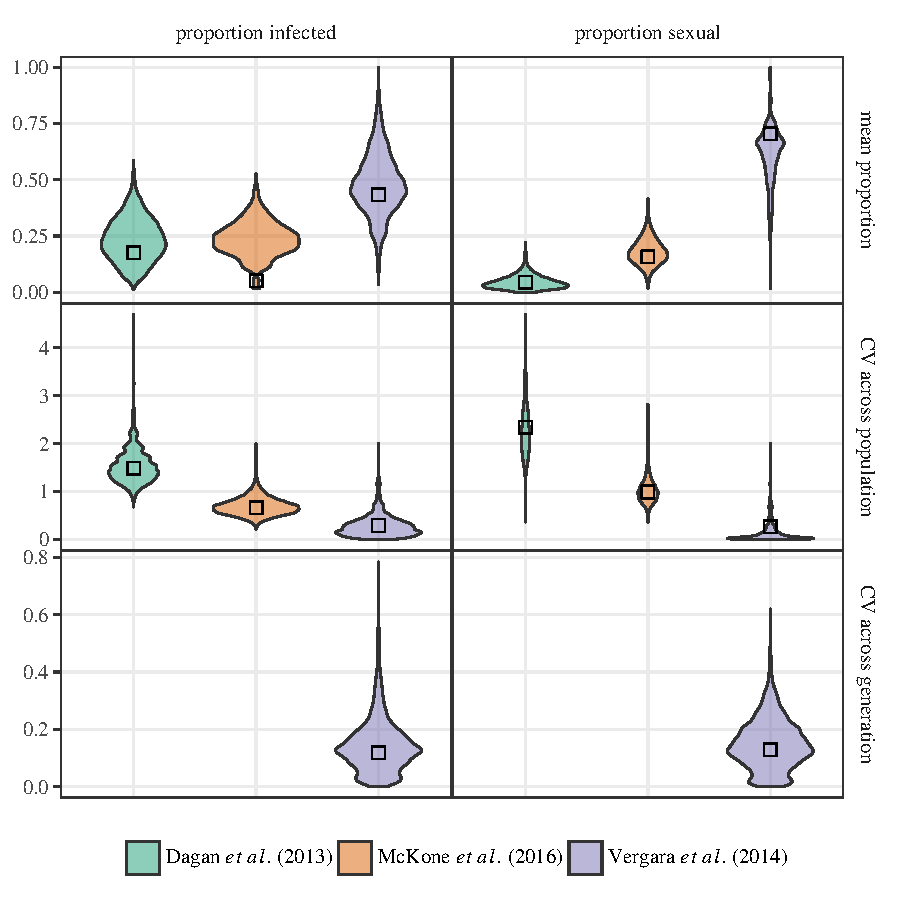
\includegraphics[width=\textwidth]{../fig/smc_summary.pdf}
\caption{{\bf Summary statistics of the observed data vs. distribution of summary statistics of the simulated data from the posterior samples.}
Dotted horizontal lines represent observed summary statistics calculated from the data.
Violin plots show the weighted distribution of fitted summary statistics (i.e., summary statistics that were accepted during ABC);
they represent the uncertainty in the estimate of the true values.
Error bars show 95\% weighted quantiles of predicted summary statistics;
they are wider than the distribution of the fitted values because they account for the uncertainty in the full distribution of the Red Queen dynamics from the estimated parameter values.
The weights correspond to the posterior distribution weights from ABC.
For each posterior sample, 10 simulations are run and each simulated system is sampled at random 100 times so that each sample consists of the same number of populations as in the fitted data.
All univariate summary statistics are matched reasonably well, except for the mean proportion of infected hosts in \cite{mckone2016fine} (indicated by an asterisk). 
}
\label{fig:smcsumm}
\end{figure}

To further diagnose the fit, we compare the predicted relationships between the mean proportion of infected hosts and the mean proportion of sexual hosts across subpopulations with the observed data (\fref{ivs}).
This is done by simulating the metapopulation model multiple times from the estimated parameters and calculating the mean proportion of infected and sexual hosts for each subpopulation from each simulation.
Then, a two dimensional distribution of these means is compared with the observed proportions.
If our model is able to sufficiently capture the observed dynamics, we would expect the observed data points to fall within high density regions.
Since we plot the \emph{predicted} densities, they are able to capture the full range of coevolutionary dynamics, which may be only partially represented in the observed data.

Despite its accuracy in reproducing summary statistics reported by \cite{dagan2013clonal}, 
our model poorly captures the relationship between the mean proportion of infected hosts and the mean proportion of sexual hosts (\fref{ivs}; \cite{dagan2013clonal}).
The model predicts sexual reproduction to be well maintained when infection prevalence is high ($> 40\%$) whereas
the observed data \citep{dagan2013clonal} suggests that sexual reproduction can only be supported when infection prevalence is low ($< 20\%$).
\cite{mckone2016fine} also found sexually reproducing snails in sites with low infection prevalence ($< 20\%$);
we note that infection prevalence may underrepresent the strength of parasite-mediated selection as
infected \textit{P. antipodarum} experiences higher risk of predation from ducks to complete the life cycle of \textit{Microphallus} \citep{levri1996effects}.
\swp{added the last sentence as suggested by Lively}

On the other hand, \citetapos{vergara2014infection} data set suggests that sexually reproducing subpopulations are likely to have a relatively high prevalence of infection across several years (approximately 20\% - 80\%).
This observation is broadly consistent with our model prediction --  
most of the data points fall within the range of model predictions (\fref{ivs}; \cite{vergara2014infection}).
However, there is one site in which more than 90\% of the snails were found to be sexual throughout the study period of 5 years \citep{vergara2014infection};
our model fails to maintain such high levels of sexual reproduction.

\begin{figure}[!ht]
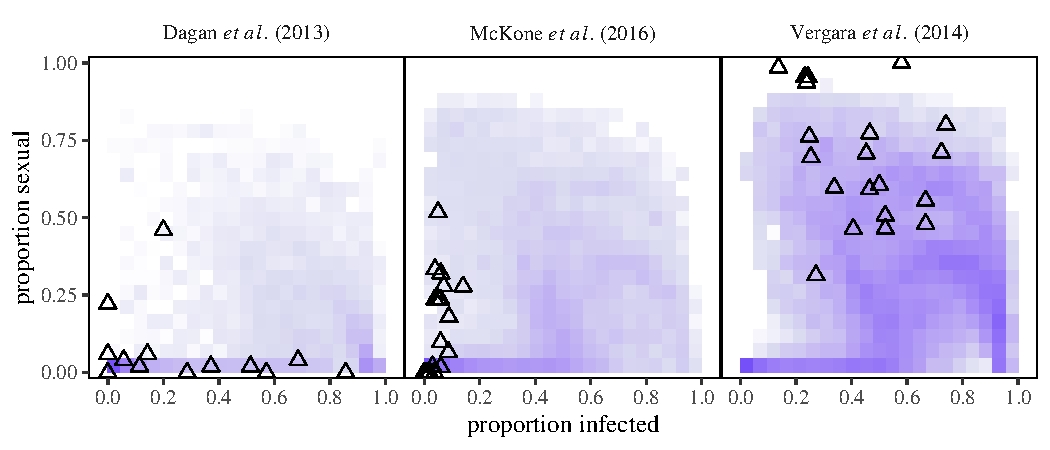
\includegraphics[width=\textwidth]{../fig/simulated_data2.pdf}
\caption{{\bf Predicted relationship between mean infection prevalence and mean proportion of sexual hosts in each population.}
For each posterior sample, 10 simulations are run.
For each population within a simulation, mean infection prevalence and mean proportion of sexual hosts is calculated by averaging across last two generations (assuming that one year contains two snail generations \citep{neiman2005variation}).
Each point, consisting of mean infection prevalence and mean proportion of sexual hosts, is assigned the weight of the parameter used to simulated the population.
The density at each cell is calculated as the sum of weights of the points that lie within it.
Cell densities are normalized by dividing by the maximum grid densities for each fit.
Dashed contours are calculated at $\log(\textrm{normalized density}) = -4$ to distinguish low- and high-density regions.
Open triangles represent the observed data (proportion of sexual hosts is computed by doubling proportion of male hosts).
For brevity, we compare data points from \cite{vergara2014infection}, which represent 5 years of Red Queen dynamics, with data points from simulations averaged across 2 last generations, which effectively represent 1 year of Red Queen dynamics;
because we calculate the densities across 1000 simulations, we expect the distribution of the simulated points to sufficiently capture the range of spatiotemporal dynamics of the Red Queen cycles.
}
\label{fig:ivs}
\end{figure}

There is a high posterior density region in which the proportion of infected hosts remains almost constant (around 0.5) among subpopulations while the proportion of sexual hosts can range from 0 to 0.3 (visible in the fits to \cite{mckone2016fine}).
As transmission rate ($\beta$) increases, selection for sexual hosts increases but the increasing number of resistant offspring prevents further infection from occurring and can decrease overall infection prevalence.
This trend is consistent with previous results of \cite{lively2001trematode} who noted that there is a region in which either sexual and asexual reproduction can be selected exclusively under the same infection prevalence.

Our model fit to \cite{vergara2014infection} predicts that the proportion of sexual hosts will decrease as infection prevalence becomes extremely high (see the shape of the contour lines in \fref{ivs}: \cite{vergara2014infection}).
This pattern can be explained by the decrease in fitness of sexual hosts with the increase in infection prevalence, predicted by \cite{ashby2015diversity}.
The same pattern can be seen in earlier work by \cite{lively2010epidemiological}.

\fref{smcparam} presents parameter estimates.
Keeping in mind that we do not obtain good fits to data from \cite{dagan2013clonal} and \cite{mckone2016fine}, we still find that high virulence and a low ratio of asexual to sexual genetic diversity are necessary to explain the observed dynamics.
Moreover, we are able to capture observed differences in mean and variation in infection prevalence among studies in our estimates of transmission rate parameters ($\beta_{\textrm{\tiny mean}}$ and $\beta_{\textrm{\tiny CV}}$).

Our fits to \cite{mckone2016fine} suggest that the scale parameter for the cost of sex, $c_b$, should be higher than our prior assumption based on \cite{gibson2017two} that estimated the cost of sex to be 2.14 (95\% CI: 1.81 - 2.55).
\cite{ashby2015diversity} defined $c_b$ as additional costs and benefits of sex, where $c_b=1$ corresponds the two fold cost.
Under their interpretation, our estimate of $c_b$ corresponds to a slightly lower estimate of the cost of sex: 1.95 (95\% CI: 1.68 - 2.4). 
(We propose an alternate interpretation to this parameter estimate below).

\begin{figure}[!ht]
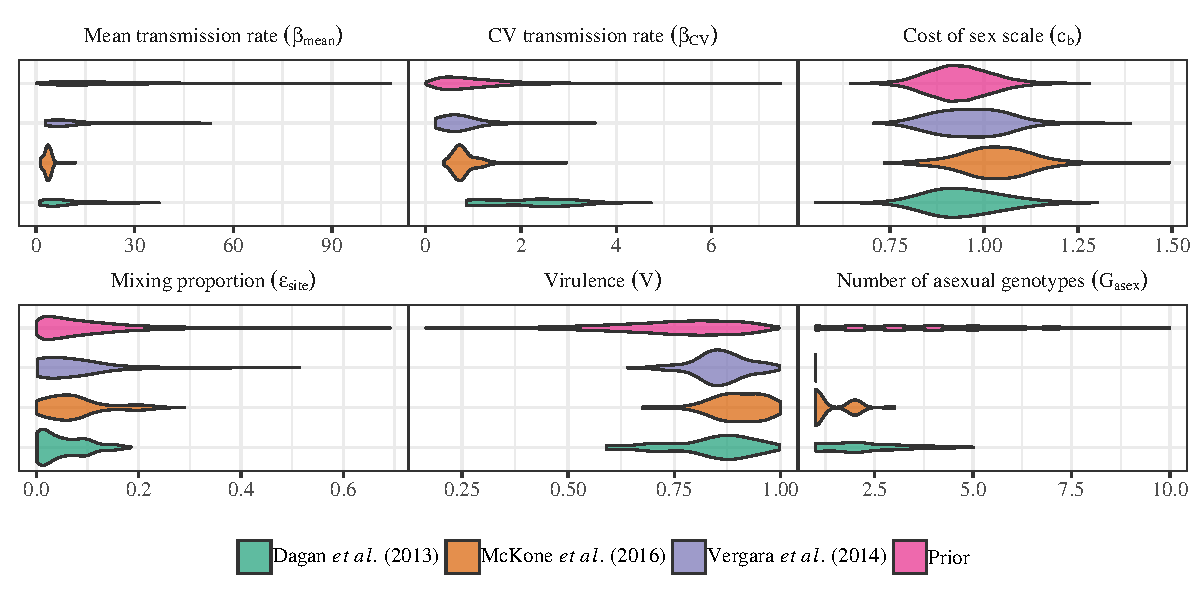
\includegraphics[width=\textwidth]{../fig/posterior.pdf}
\caption{{\bf Parameter estimates from Sequential Monte Carlo Approximate Bayesian Computation.}
We estimate mean transmission rate ($\beta_{\textrm{\tiny mean}}$), CV in transmission rate ($\beta_{\textrm{\tiny CV}}$), virulence ($V$), mixing proportion ($\epsilon_{\textrm{\tiny mean}}$), number of asexual genotypes ($G_{\textrm{\tiny asex}}$), and a scale parameter for cost of sex ($c_b$).
Violin plots represent weighted distribution of 100 posterior samples obtained from ABC.
Violin plots for prior distribution is obtained by drawing 10000 random parameter samples from the prior distribution.
$G_{\tiny \textrm{asex}}$ is a discrete variable but is drawn on a continuous scale for convenience.
See Table~\ref{tb:param} for full parameter descriptions and their prior distributions.
}
\label{fig:smcparam}
\end{figure}

Finally, our power analyses suggest that there is high power to detect a positive correlation between infection prevalence and frequency of sexual hosts in the systems studied by \cite{dagan2013clonal} and \cite{mckone2016fine} (\fref{power}).
Such high power predicted for \cite{dagan2013clonal} is particularly surprising given that they were not able to observe the expected correlation.
This discrepancy implies that the snail-trematode system studied by \cite{dagan2013clonal} show sufficient variation in infection prevalence in order for the correlation to be observed under pure Red queen selection, but other underlying factors that are neglected by our model may have caused the system to deviate from their expected behaviors (predicted by Red Queen models);
in particular, only 2 out of 22 populations contains sexual snails.
On the other hand, our model predicts low power for detecting the positive correlation for the system studied by \cite{vergara2014infection} (\fref{power}).

Overall, our analysis suggests that increasing the number of study sites is a more effective way to increase power than increasing the number of samples per site (\fref{power}).
The correlation between the proportion of infected and sexual hosts depends on the spatial distribution of parasite infection; 
increasing the number of sites can help us better capture this distribution and increase the power to observe the correlation.
On the other hand, collecting more samples from a site only gives us a more accurate estimate of the two proportions for that specific site; it does not tell us how these proportions are distributed across space.
As a result, the power quickly saturates once we have a sufficient number of samples ($> 100$) to estimate the two proportions reliably at each site.

While we originally planned to perform power analysis using Spearman's rank correlation,
we repeated the analysis using Pearson's correlation after applying arcsine square root transformation \citep{lively1992parthenogenesis} to see whether this procedure improves power.
Using Pearson correlation (with transformation) gives slightly higher power to detect the positive correlation between frequency of sexual hosts and infection prevalence (see Appendix).

\begin{figure}[!ht]
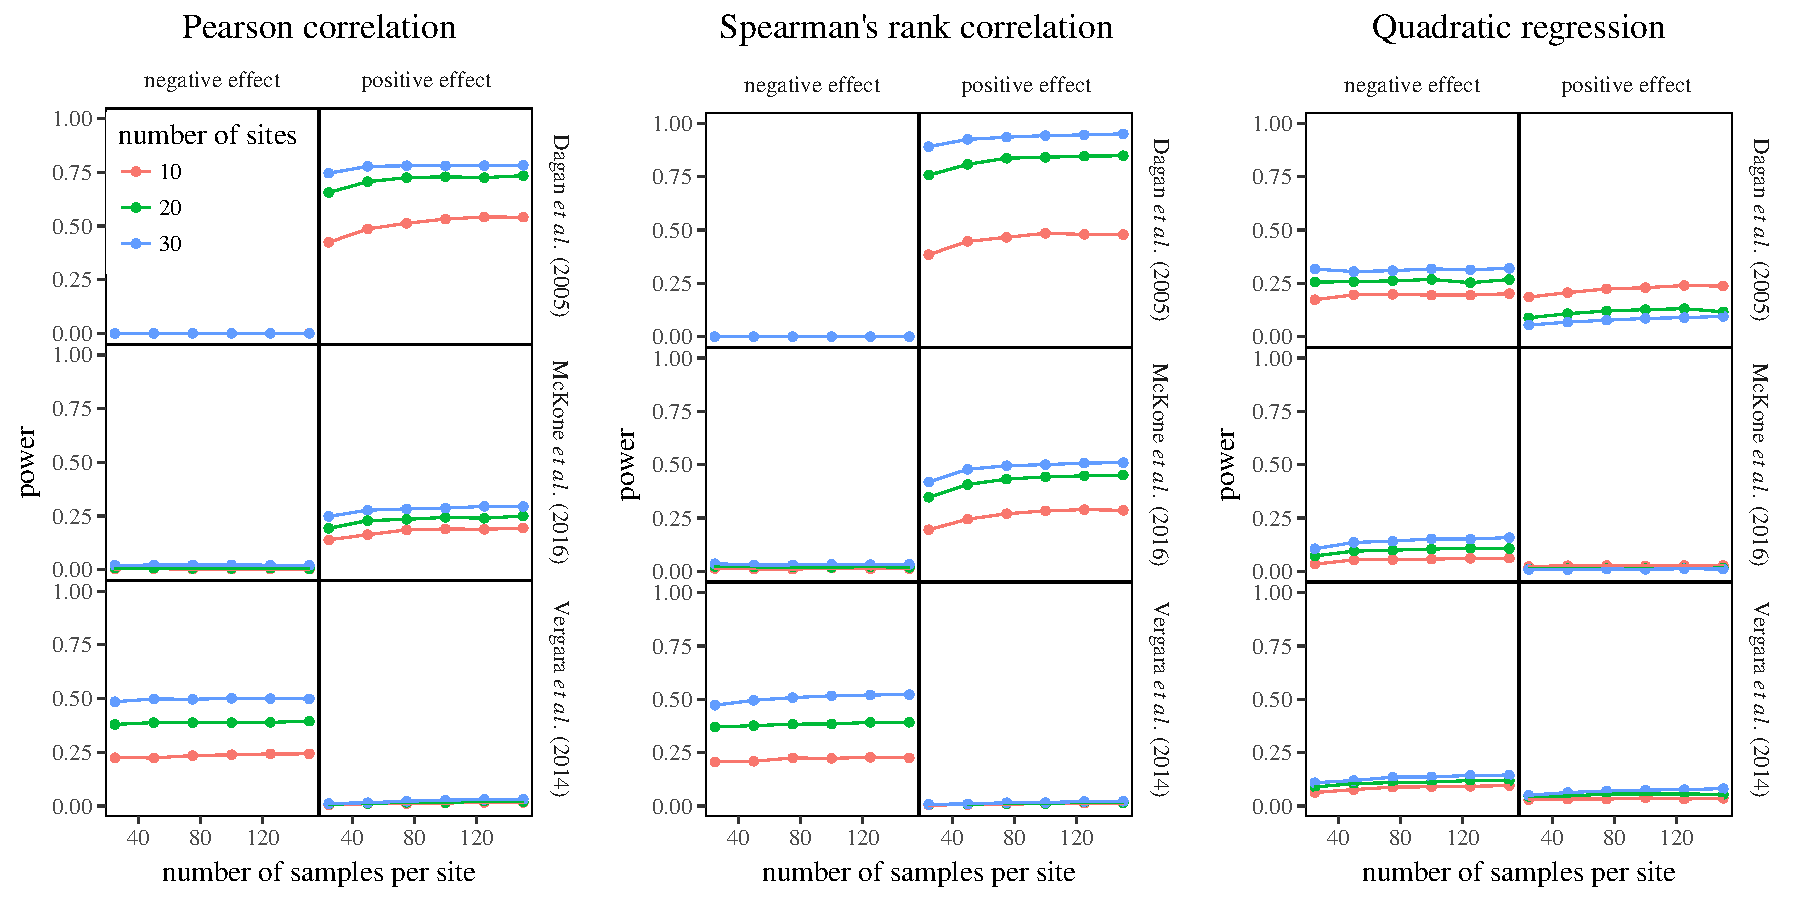
\includegraphics[width=\textwidth]{../fig/power.pdf}
\caption{{\bf Power to detect a statistically significant positive correlation between infection prevalence and frequency of sexual hosts.}
Spearman's rank correlation was used to test for correlation between infection prevalence and frequency of sexual hosts in simulated data from the posterior distributions.
}
\label{fig:power}
\end{figure}

\section{Discussion}

\rev{remind the reader of the biologically meaningful parameters.}
\swp{I tried to reword this paragraph}
We compared summary statistics (mean and coefficient of variation in proportion of infected
and sexual hosts) of model simulations and those of the observed 
data using Approximate Bayesian Computation (ABC) to infer biologically realistic 
range of model parameters, which reflects the observed Red Queen dynamics (\fref{smcparam}).
Using the estimated parameters, we calculated the power to observe a significant,
positive correlation between the proportion of infected hosts and the proportion 
of sexual hosts (\fref{power}), as predicted by \cite{lively1992parthenogenesis}.
While our simple metapopulation coevolutionary model is able to match 
the observed prevalence of sexual reproduction and trematode infection 
across multiple snail populations (\fref{smcsumm}),
it fails to capture some of the more detailed patterns in the data (\fref{ivs});
in particular, our model (1) overestimates the required level of infection prevalence
to promote sexual reproduction and (2) is unable to match low levels of sexual reproduction 
observed by \cite{dagan2013clonal}.
These discrepancies between the model predictions and observed data suggest that a 
simple host-parasite coevolutionary model may not be able to sufficiently explain 
the maintenance of sexual reproduction observed in nature (\fref{ivs}).
\lively{This is not clear to me.  The fit seems good for Vergara et al, but not
for the Israeli snail.  So it is not clear if you are speaking about the 
difference between studies, or some kind of average over all studies.}
\swp{Tried to clarify this.}

A model that fits poorly can still provide useful information about a biological
system by challenging our model assumptions;
for example, lack of fit in dynamicsl systems (modeled by ordinary differential 
equations) can suggest misspecification of a model on various levels, including
rate equations governing the dynamics of a system and their relevant state variables
\citep{hooker2015goodness}.
Our model clearly failed to match the data presented by \cite{dagan2013clonal} (\fref{ivs}).
The snail-trematode system studied by \cite{dagan2013clonal} live in qualitatively different environments from the New Zealand system that we considered \citep{vergara2014infection, mckone2016fine}.
For example, their habitats are subject to seasonal flash floods, which can act as 
strong bottlenecks and promote asexual reproduction \citep{ben2007temporal}.
Because our model did not account for these details, it failed to match the observed 
relationship betweens infection prevalence and frequency of sexual reproduction;
nonetheless, lack of fit of a simple Red Queen model to this data does not exclude the 
possibility that sexual reproduction is maintained by parasite selection in this 
system.
% These results suggest that a significant correlation (or the lack of it) between infection prevalence and the frequency of sexual reproduction may not provide sufficient evidence for (or against) the role of parasites in maintaining sexual reproduction in the host population.

The model fits to \cite{dagan2013clonal} and \cite{mckone2016fine} suggest that the cost of sex can be overcome and sexual reproduction can be maintained only if infection prevalence is much higher than the observed prevalence (\fref{ivs}).
In other words, the benefit of producing offspring with novel genotype is relatively small when infection prevalence is low.
In order to support sexual reproduction at lower infection prevalence, the benefit of sex must be greater or other mechanisms must compensate for the difference.
As our model relies on a simple structure and strong parametric assumptions, an additional benefit of sex can only be provided by lowering the cost of sex (i.e., increasing the scale parameter, $c_b$).

The simple structure of the model and limited genetic diversity can explain the discrepancy between model prediction and the observed data by \cite{mckone2016fine}.
Here, we assumed that host resistance to infection is determined entirely by two biallelic loci, resulting in 10 possible genotypes.
However, it is unlikely that such a simple model can capture the genetic interaction between hosts and parasites observed in nature.
Although exact genetic architecture that determines trematode infection in snails (e.g., the number and inheritance of loci involved in parasite resistance) is not known, the documented genetic diversity of snails is far greater than what our model assumes \citep{fox1996genetic, king2011parasites, dagan2013clonal}.
Increasing the maximum possible genetic diversity of the model would have allowed sexual hosts to escape infection more easily and maintained sexual reproduction at a lower prevalence of infection \citep{lively2010effect, king2012does, ashby2015diversity}.

While the positive correlation between frequency of sexual hosts and prevalence of infection can provide evidence for the effect of the parasite on the maintenance of sexual reproduction in the host population, it does not fully capture the coevolutionary process.
In particular, the positive correlation represents a contrast between populations that undergo Red Queen dynamics and those that do not (rather than a continuous relationship between the frequency of sexual hosts and prevalence of infection):
low-risk populations will be dominated by asexual individuals whereas high-risk populations will consist of both sexual and asexual individuals.
\cite{lively2001trematode} gave a similar explanation and predicted that large variation in the risk of infection is required to observe the predicted correlation.

The similarity between the correlations predicted by the model and the correlations observed in nature may provide us more confidence that the observed populations provide evidence for the Red Queen Hypothesis (\fref{effect}).
However, the strength of the correlation is not a direct measure of the strength of selection imposed on the host population.
Moreover, when populations are actively coevolving, wide range of correlations can be detected (\fref{effect}: \cite{vergara2014infection}).
While simple statistical summaries, such as a correlation coefficient, are easily accessible,
more sophisticated and mechanistic statistical models that yield biologically interpretable parameters may be better suited for understanding the effect of parasites on the maintenance of sexual reproduction in the host population.

\begin{figure}[!ht]
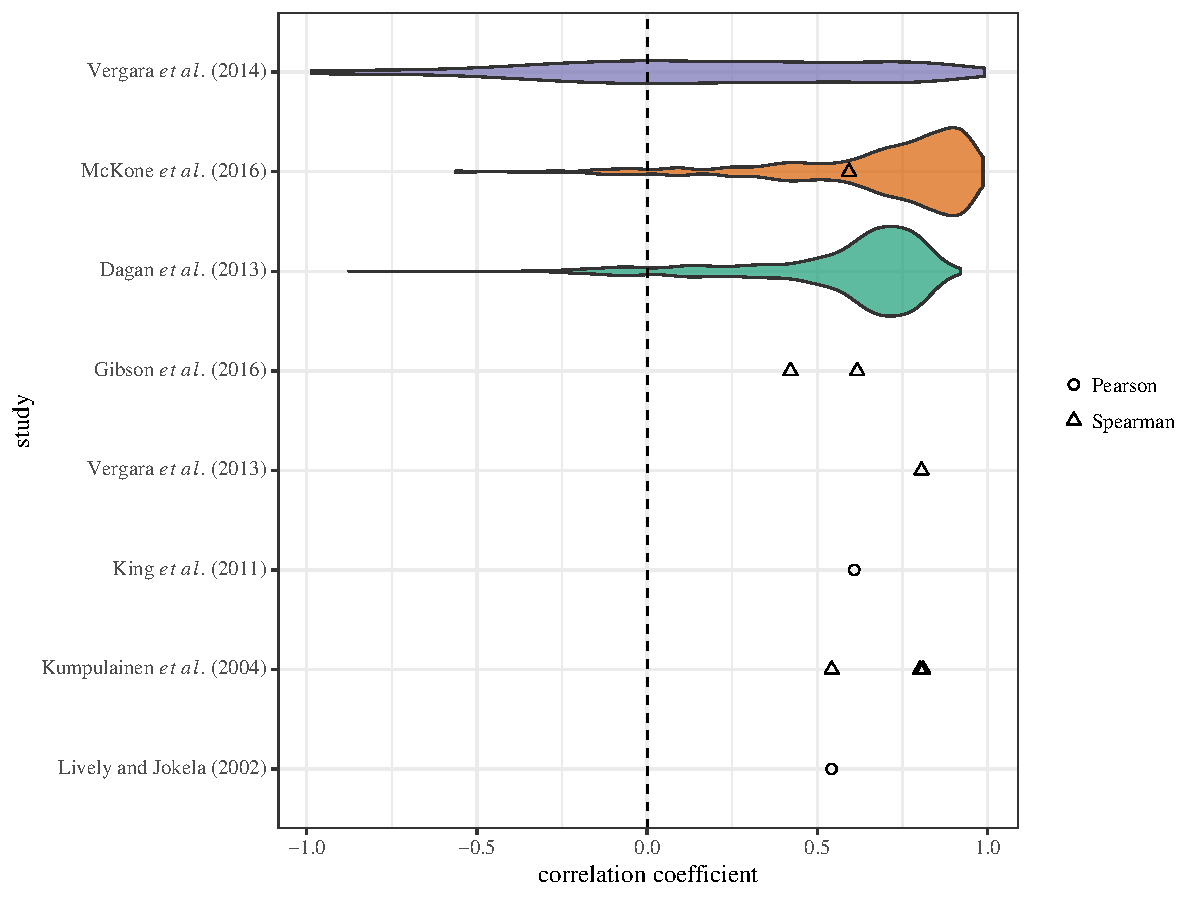
\includegraphics[width=\textwidth]{../fig/effect_size.pdf}
\caption{{\bf Predicted vs. observed correlation between infection prevalence and frequency of sexual hosts.}
Violin plots show weighted distribution of predicted strength of correlation based on ABC fits.
Predicted correlation was measured for each simulation from the posterior by taking into account the last two generations from each simulated population.
Triangles and circles represent observed correlation sizes from previous studies.
\cite{dagan2013clonal} and \cite{vergara2014infection} do not report the size of the correlation; correlations are re-calculated from their data sets using both Pearson (after applying arcsine square root transformation) and Spearman correlations.
}
\label{fig:effect}
\end{figure}

Mathematical models have used extensively to build theoretical foundations for the evolution of sex but only a few models have been confronted with data.
The idea of the two-fold cost of sex was only recently tested directly by fitting a theoretical model to observed data \citep{gibson2017two}.
Making statistical inference on the observed systems and testing theoretical models against data may provide deeper insight into underpinnings of maintenance of sexual reproduction.

\section{Acknowledgements}

We thank SHARCnet for providing computational resources, and Curtis Lively, Yannis Michalakis, and an anonymous reviewer for helpful comments. 

\section{Funding}

This work is supported by The Natural Sciences and Engineering Research Council, Undergraduate Student Research Award (to SWP).

\bibliography{redqueen}

\pagebreak
\section*{Appendix}

\renewcommand\thefigure{A\arabic{figure}}    
\setcounter{figure}{0}   

\begin{figure}[!ht]
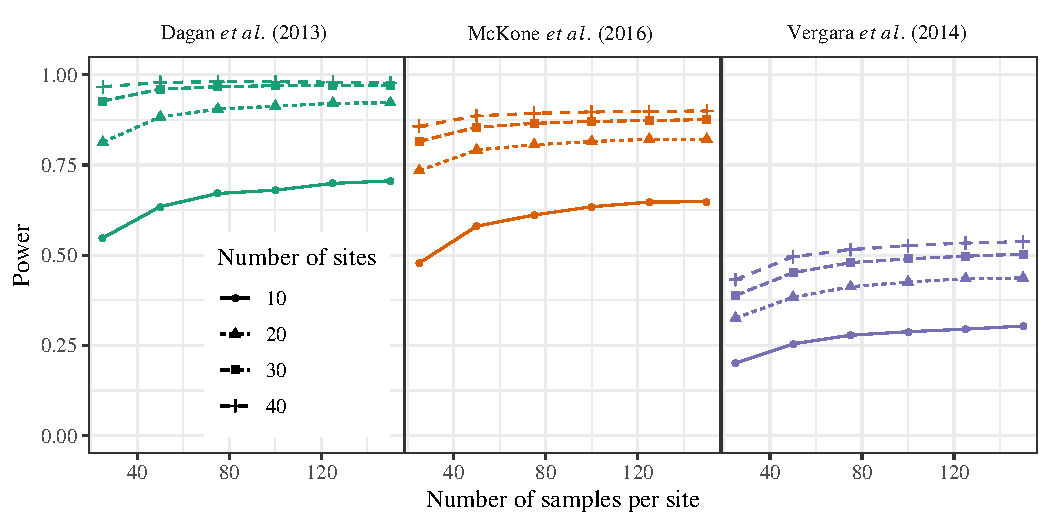
\includegraphics[width=\textwidth]{../fig/power_lm.pdf}
\caption{{\bf Power to detect a statistically significant positive correlation between infection prevalence and frequency of sexual hosts.}
Pearson correlation was used to test for correlation between square root arcsine transformed infection prevalence and frequency of sexual hosts in simulated data from the posterior distributions.
}
\label{fig:power_lm}
\end{figure}

\end{document}
